\section{Anomaly detection method}
\label{sec-anom}

In this paper, we are detecting anomaly on labelled dataset. For this problem, we are considering  each gene expression consists of same number of time points. Therefore, the value of the time points are working as feature vector of the gene expressions. For example, for a gene expression $g_i=\{x_1,x_2,x_3,\dots,x_T$\}, $x_1,x_2,\dots x_T$ are its feature values. Since these time points are sequential and related with previous values, traditional feature based machine learning methods are not satisfactory for them. We propose deep learning based Convectional Neural Network (CNN) and Long Short Term Memory (LSTM) approach. In order to evaluate the performance of these techniques we also apply traditional supervised and unsupervised machine learning algorithms on this classification. 

\subsection{Convolutional Neural Network (CNN)}

\begin{figure*}
    \centering
    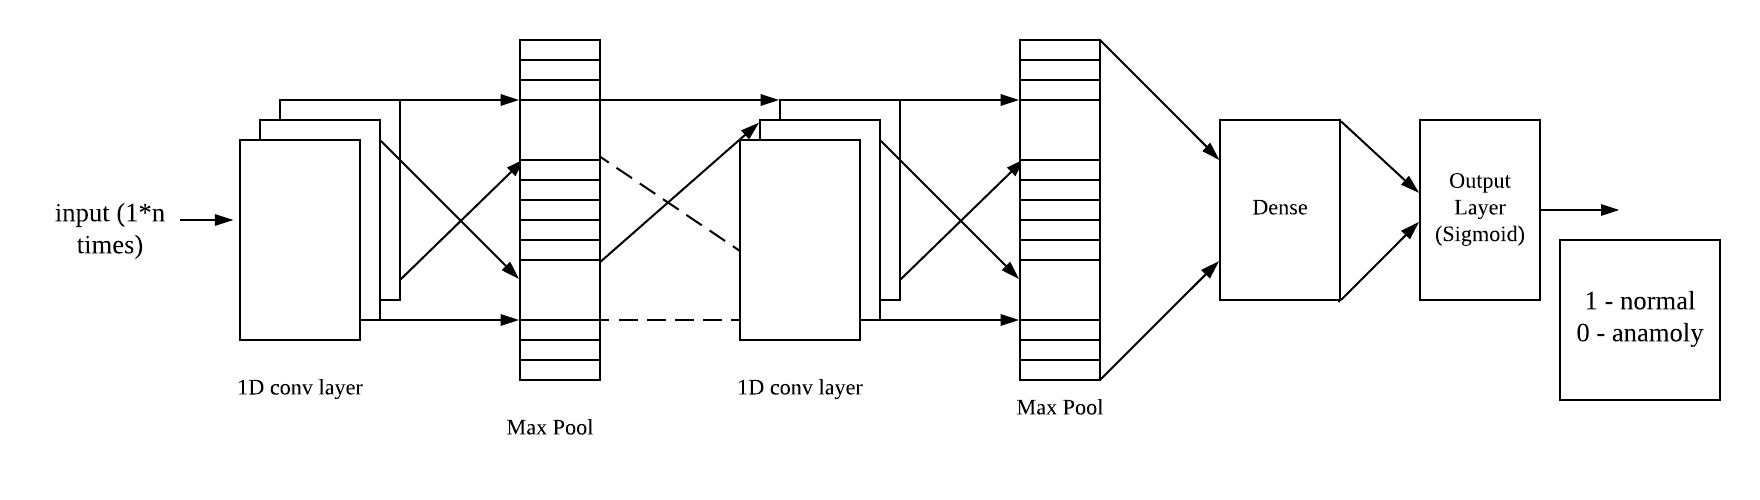
\includegraphics[height=4cm]{Figures/CNN.png}
    \caption{CNN Architecture}
    \label{fig:cnn}
\end{figure*}
Initially we resize the gene expression as matrix form to feed into  the convolutional layer. The convolutional layers are constructed using one-dimensional kernels that move through the sequence (unlike images where 2d convolutions are used). These kernels act as filters which are being learned during training. As in many CNN architectures, the deeper the layers get, the higher the number of filters become. Each convolution is followed by pooling layers to reduce the sequence length. 

Once the last layer is reached, we need to flatten the tensor and feed it to a classifier with the right number of neurons and therefore use a fully connected layer. Then, the classifier outputs the class of gene expression and sigmoid is used as activation function since one neuron is enough to provide the output.  We  use dropout regularization to prevent over-fitting and   use  Adam optimizer. We use a batch size of 32 in our training process. 

\subsection{Long Short Term Memory (LSTM)}
\begin{figure*}
    \centering
    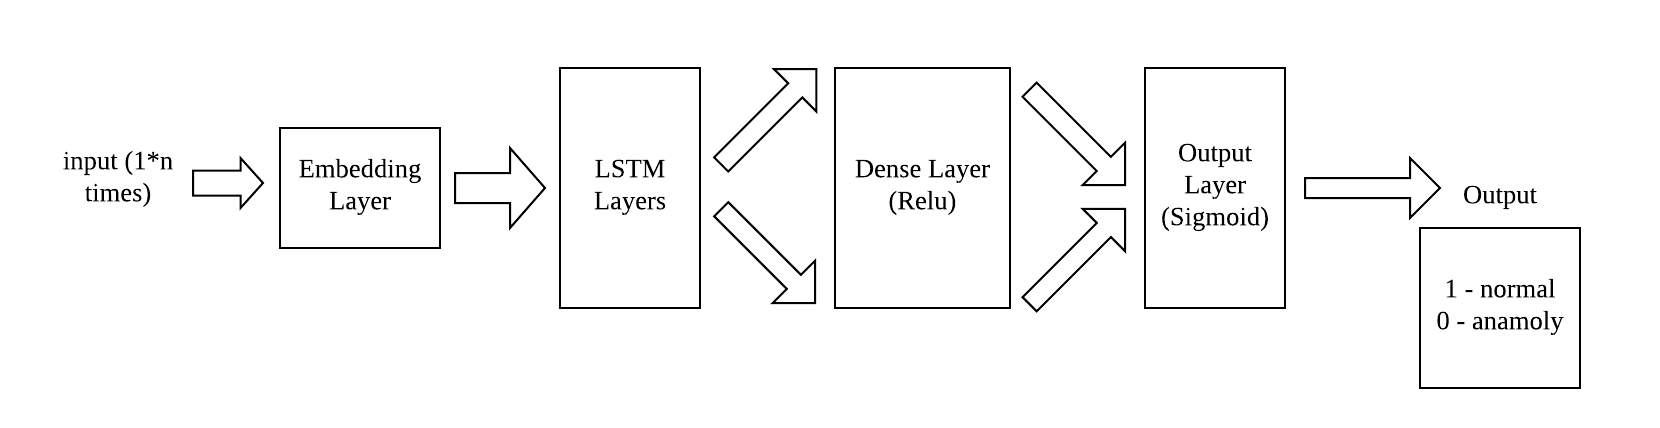
\includegraphics[height=4cm]{Figures/LSTM.png}
    \caption{LSTM Architecture}
    \label{fig:lstm}
\end{figure*}

In this method, we resize the gene expressions and feed them  into the embedding layer with no initial weights. The features are given weights in this layer and then provided to a basic LSTM layer with 200 cells. Then we add a dense layer with Relu activation. Finally sigmoid is used as activation function in the output layer. Output 0 means anomalous and 1 means normal gene expression in our problem.

\subsection{Supervised method: SVM}
Support Vector Machine (SVM) is a discriminative classifier formally defined by a separating hyperplane. In other words, given labeled training data (supervised learning), the algorithm outputs an optimal hyperplane which categorizes each data points. In two dimentional space this hyperplane is a line dividing a plane in two parts where in each class lay in either side. In this method, we ploted feature value of time series in x-axis and output level in y-axis (1/0 for normal/anomaly). Then svm finds out a line/hyper-plane that separate outs both classes. Very importrant characteristic of SVM classifier is margin. Margin is a separation of line to the closest class points. A good margin is one where this separation is larger for both the classes. For good margin of kernel, we used $L_2$ loss.


\subsection{Unsupervised method: One class SVM}
One-Class SVM has been introduced by Schölkopf et al.\cite{one_svm}.
It tries to learn a rough, close frontier delimiting the contour of the initial observations distribution, plotted in embedding d-dimensional space. Then, if further observations lay within the frontier-delimited subspace, they are considered as coming from the same population than the initial observations. Otherwise, if they lay outside the frontier, we can say that they are anomaly with a given confidence in our assessment.

 It requires the choice of a kernel and a scalar parameter $\nu$ to define a frontier.  The $\nu$ parameter, also known as the margin of the One-Class SVM, corresponds to the probability of finding a new, but regular, observation outside the frontier. We use the default RBF kernel and set $\nu$ to 0.1.





